\section{Connectedness}

Again, fix a topological space $X$. In this section, we discuss different notions of connectedness of a toplogical space.

\begin{boxdefinition}[Disconnectedness]
    We say a space $X$ is \textbf{disconnected} if there exist disjoint (nonempty) open sets $U, V \subset X$ with $U \cup V = X$. If $U$ and $V$ are disjoint and cover $X$, we say that they \textbf{disconnect $X$}.
\end{boxdefinition}

We similarly say that $A\ssq X$ is disconnected if $A$ is disconnected as a space endowed with the subspace topology inherited from $X$.

\begin{boxwarning}
     One must be very careful when disconnecting sets: \textbf{when you have a disconnected set} $A\ssq X$, it is not at all obvious that the sets you use to disconnect $A$ (namely, $U$ and $V$) are actually disjoint in the rest of $X$.\\
     
     Remember this for your General Topology basic exam!
\end{boxwarning}

We can use this definition to define connectedness in the obvious way.

\begin{boxdefinition}[Connectedness]
    We say $X$ is \textbf{connected} if $X$ is not disconnected, ie, if there do not exist disjoint open sets $U$ and $V$ that disconnect $X$.
\end{boxdefinition}

As one would expect, we define connectedness for subsets to be connectedness with respect to the subspace topology.

It turns out we can use the definition of connectedness to say something about the clopen sets of a connected space.

\begin{boxlemma}
    Let $\parenth{A_i}_{i \in \I}$ be some family of subsets of $X$ indexed by some non-empty set $\I$ such that
    \begin{enumerate}
        \item For all $i \in \I$, $A_i$ is a connected subset of $X$
        \item For all $i, j \in \I$, $A_i \cap A_j \neq 0$
    \end{enumerate}
    That is, $\parenth{A_i}$ is a family of connected, \textit{non-disjoint} sets. Then,
    \begin{align*}
        A := \bigcup_{i \in \I} A_i
    \end{align*}
    is a connected subset of $X$.
\end{boxlemma}
\begin{proof}
    Suppose that $A$ is not connected. Then, there exist open subsets $U, V \subsetneq X$ such that
    \begin{align*}
        A = \parenth{A \cap U} \cup \parenth{A \cap V}
    \end{align*}
    with $\parenth{A \cap U}$ and $\parenth{A \cap V}$ being disjoint, non-empty, and proper subsets of $A$. Then, for any $i \in \I$, we have that
    \begin{align*}
        A_i \subseteq A = \parenth{A \cap U} \cup \parenth{A \cap V}
    \end{align*}
    Since the $A_i$ are all connected, we know that for all $i \in \I$, either $A_i \ssq U$ or $A_i \ssq V$. It turns out that we can do better: either every $A_i$ is contained in $U$ or every $A_i$ is contained in $V$. Indeed, if this were not the case, then there would be $i, j \in \I$ with $A_i \in U\cap A$ and $A_j \in V\cap A$. 
    
    Since $U\cap A, V\cap A$ are disjoint this would imply $A_i\cap A_j=\emptyset$ (a contradiction), from which it follows that we must have either every $A_i$ is contained in $U$ or every $A_i$ is contained in $V$.

    Without loss of generality, say that every $A_i$ is contained in $U$. Then, $A \ssq U$ also, meaning that $A \cap U = A$. Hence, $A \cap V = \emptyset$, which contradicts the assumption that $A$ is disconnected, because disconnecting subsets must be proper.
\end{proof}

 We next use the definition of connectedness to establish a ``canonical'' decomposition of $X$.

 \subsection{Connected Components}

 Define the binary relation $\sim$ on $X$ such that $a \sim b\iff \exists A\subseteq X$ with $A$ connected and $a,b \in A$. We then claim that $\sim$ is an equivalence relation, and (having shown this with reference to the previous lemma) we let the equivalence classes of $\sim$ partition $X$ into sets $X_i$.
 %probably don't want this as the definition, feel free to delete
 % Isn't this what we'd want as the definition? hmm
 %or as maximal connected components, idk - yes, as the maximal connected sets of the sapce X (anything works?)
 % An equivalence class is always maximal in the set of things related to any representative... but if you mean the maximal connected set containing it then idk. 
 \begin{boxdefinition}[Connected Components]
     The \textbf{connected components} of $X$ are the equivalence classes in $\quotient{X}{\sim}$, with $\sim$ being defined as above.
 \end{boxdefinition}

Let us describe these equivalence classes. Fix $x \in X$. Denote its equivalence class in $\quotient{X}{\sim}$ by $\brac{x}$. Then, it is possible to show that
\begin{align*}
    \brac{x} = \setst{y \in X}{y \sim x} = \bigcup\setst{A \ssq X}{x \in A \text{ and } A \text{ is connected}}
\end{align*}
The $\ssq$ inclusion is clear, because $\brac{x}$ is itself connected, meaning that any $y \in \brac{x}$ clearly lies in some connected subset of $X$ containing $x$. Conversely, any element of any connected subset of $X$ containing $x$ must be connected to $x$, putting it in $\brac{x}$.

\begin{boxlemma}\label{Ch1:Lemma:closure_connected_connected}
    If $A \ssq X$ and $A$ is connected, then $\closure{A}$ is also connected.
\end{boxlemma}
\begin{proof} % This is actually not really a true proof by contradiction. In fact, even in the most constructive of type theories, I am quite sure that the definition you'd want to implement for connected is "not disconnected". The definition of "not P" is always "P implies False", which you can prove (constructively) by assuming P and deducing False (ie, "proof by contradiction"). A true proof by contradiction uses LEM in the way that it's set up, which this does not.
    Suppose that $\closure{A}$ is not connected. then, there are open sets $U, V \ssq X$ such that $\closure{A} \ssq U \cup V$, $(\closure{A} \cap U)\cap (\closure{A}\cap V) = \emptyset$, and $\closure{A} \cap U, \closure{A} \cap V \neq \emptyset$.  We can see, since $A \ssq \closure{A}$, that $A = \parenth{A \cap U} \cup \parenth{A \cap V}$, with $A \cap U \cap V = \emptyset$. It follows that $A\cap U, A\cap V$ disconnect $A$ (and the result now follows either from contrapositive or contradiction depending on what you're feeling today). %\sorry % Simply show containment in complement
\end{proof}

\begin{boxcorollary}
    The connected components of $X$ are closed subsets of $X$.
\end{boxcorollary}
\begin{proof}
    Fix $x \in X$. Then, by \Cref{Ch1:Lemma:closure_connected_connected}, the closure $\closure{\brac{x}}$ of the connected component $\brac{x}$ containing $X$ is a connected subset of $X$. Since all such connected sets are contained in $\brac{x}$, we have that $\closure{\brac{x}} \ssq \brac{x}$, meaning $\brac{x}$ is equal to its closure, making it closed.
\end{proof}

\subsection{Preserving Connectedness}

Surprisingly---or unsurprisingly---connectedness is not preserved by taking subsets.

\begin{boxcexample}[A Disconnected Subset of a Connected Space]
    We know that $\R$ is connected under the Euclidean topology. Consider $\Q \subset \R$. We can clearly see that $\parenth{-\infty, \sqrt{2}} \cap \Q$ and $\parenth{\sqrt{2}, \infty} \cap \Q$ are disjoint, open, proper subsets of $\Q$ that disconnect it.
\end{boxcexample}

However, it turns out the \textit{image} of a connected set in a continuous function \textit{is} connected.

\begin{boxlemma}
    Let $X$ and $Y$ be topological spaces. Let $A \ssq X$ be connected and let $f : X \to Y$ be continuous. Then, $f[A]$ is connected.
\end{boxlemma}
\begin{proof}
    If not, let $U, V \ssq Y$ be open with $f[A]$ disconnected by $U,V$. Then we would have $A$ disconnected by $f^{-1}[U], f^{-1}[V]$ (as these sets are open and disjoint, and their union contains $A$), contradicting our assumption that $A$ is connected.
\end{proof}

This allows us to construct many examples of connected spaces.

\begin{boxexample}[Connectedness of the Unit Interval]
    Consider $\brac{0, 1}$ along with the subspace topology inherited from the Euclidean topology on $\R$. We show that $\brac{0, 1}$ is connected. \\
    
    Indeed, suppose $\brac{0, 1}$ is \textit{not} connected. Then, there exist open sets $U, V \ssq \brac{0, 1}$ such that $U \cup V = \brac{0, 1}$ and $U \cap V = \emptyset$. Thus, $0 \in U$ or $U \in V$. WLOG, say $0 \in U$. Define
    \begin{align*}
        S = \setst{a \in \brac{0, 1}}{\brac{0, a} \ssq U}
    \end{align*}
    Observe that $S$ has the following properties.
    \begin{enumerate}
        \item $0 \in S$, so $S$ is non-empty.
        \item $S$ is bounded above (by $1$, for instance)
    \end{enumerate}
    Therefore, $S$ has a finite supremum (indeed, a supremum in $\brac{0, 1}$). Denote this $b$.
    \begin{figure}[H]
        \centering
        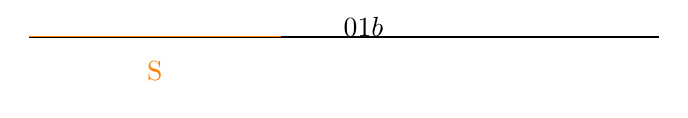
\begin{tikzpicture}[scale=4]
            \draw[black, thick] (-1, 0) -- (1, 0);

            % S
            \draw[orange] (-1, 0) -- (-0.2, 0);
            \node[label={[shift={(0,-0.8)}, orange]S}] at (-0.6, 0) {};

            % Endpoints
            \labelledpoint{-1}{0}{0}{-1}{$0$};
            \labelledpoint{1}{0}{0}{-1}{$1$};

            % b
            \labelledpoint{-0.2}{0}{0}{-1}{$b$};
        \end{tikzpicture}
        % \caption{Caption}
        % \label{fig:placeholder}
    \end{figure}
    Now, observe that $b$ has the following properties.
    \begin{enumerate}
        \item \underline{$b > 0$.} The reason for this is that since $0 \in U$ and $U$ is open, there is some $\eps > 0$ such that $\co{0, \eps} \ssq S$. Thus, $b \geq \eps > 0$.

        \item \underline{$\co{0, b} \ssq U$.} This is true by definition of $b$ and $S$.

        \item \underline{$b \in U$.} Otherwise, certainly $b \in V$, and therefore, by openness, there is some $\eps > 0$ such that $\oc{b - \eps, b} \ssq V$, but for all $\eps > 0$, we must have that $b - \eps \in U$ by definition of $b$ (and $S$), and $U$ and $V$ are disjoint.
    \end{enumerate}
    Now we note that either $b=1$ or $b\neq 1$ (by the law of excluded middle?): 
    
    If $b\neq 1$, since $U$ is open, then there exists some $\ve>0$ such that $(b-\ve, b+\ve)\ssq U$, contradicting our assumption that $b$ is the supremum of $U$. If $b=1$, but then $[0,1]\ssq U$ (by points 2 and 3) so $V$ must be empty - having reached contradiction in this instance as well, it follows that $[0,1]$
\end{boxexample}


\subsection{Path Connectedness}

\begin{boxdefinition}[Path]
    Given $X$ a space, let $a,b\in X$. We say that a \textbf{path} in $X$ is a continuous function $\gamma:[0,1]\to X$ satisfying $\gamma(0)=a, \gamma(1)=b$.
\end{boxdefinition}

% No need of `\\` in my repos because paragraph spacing is automatic.
% of course it is (thank you) :)))
\begin{remark}
    You may have many paths, be unable to use sub or super-scripts, but still need to name them all. Professor Cummings is here to help: $\alpha, \beta, \gamma, \delta, \epsilon,\zeta, \eta, \theta, \iota, \kappa, \lambda, \mu, \nu, \xi, \pi, \phi, \rho,$ etc.
\end{remark}

As a preliminary, we note that we can compose paths to obtain new paths - in other words, it can be shown that if we have a path $\alpha$ from $a$ to $b$ and a path $\beta$ from $b$ to $c$, then there is $$\gamma(t):=\begin{cases}
    &\alpha(2t):t\in [0,1/2)\\
    &\beta(2t-1):t\in [1/2, 1]
    
\end{cases}$$
forming a path from $a$ to $c$.

\begin{boxdefinition}[Path-Connected Space]
    We say that $X$ is \textbf{path-connected} iff for all $a,b\in X$ there is a path from $a$ to $b$.
\end{boxdefinition}

% Btw - keyboard shortcuts from word processors for bold/italics do work here (eg. ctrl + B encloses stuff in \textbf{})

It is possible to show that every path-connected space is connected (note that if we have nonempty $U,V$ disconnected $X$ with $a\in U, b\in V$ that there can be no path from $a$ to $b$ since $[0,1]$ is connected), but not the other way round (there's this modern art piece called the ``topologist's since curve'' you may want to look at).